\chapter{Introduction}\label{sec:intro}

In recent years, deep learning models have become larger and increasingly demand more data to perform their tasks satisfactorily. 
However, few-shot learning has garnered increasing interest recently because it underscores a fundamental gap between smart human adaptability and data-hungry supervised and unsupervised deep learning methods.

Today, machine learning models are capable of performing exceptionally well on a variety of tasks. Machine learning models already perform better than humans in several image related tasks such as object recognition, image super-resolution scaling, image analysis tasks in medicine and self-driving cars. Not only this, we have seen an explosive growth of large language models such as GPT-3 \parencite{brown2020language} and LaMDA \parencite{cohen2022lamda}, that are capable of generating coherent sentences in a manner that was previously not seen.
\begin{figure}[ht]
    \centering
    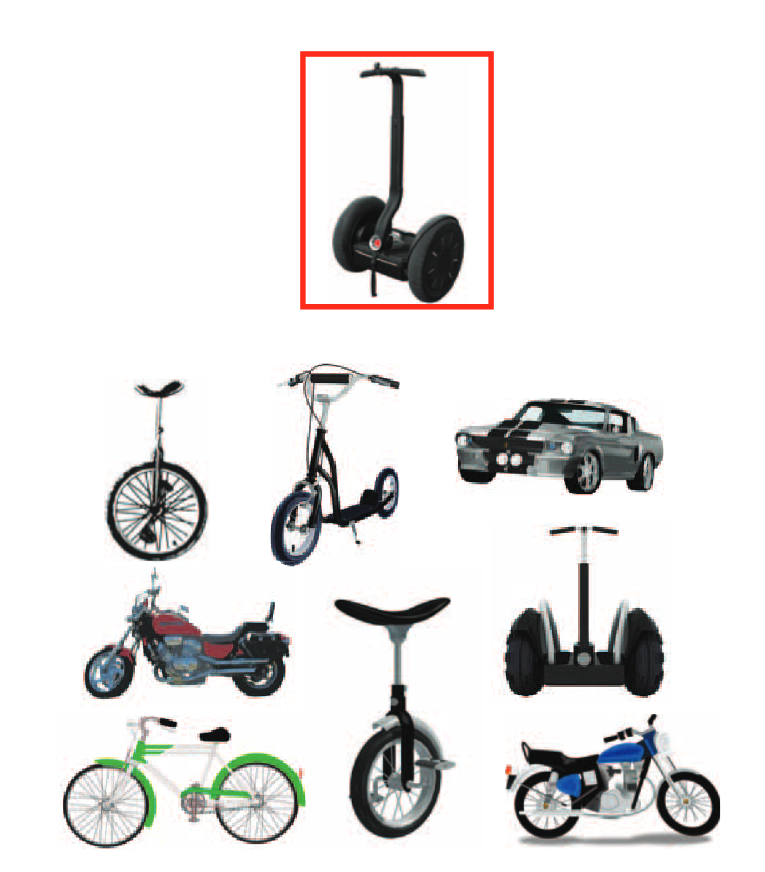
\includegraphics[scale=0.25]{chapters/assets/human-understanding.png}
    \caption{As a human one can immediately figure out which object is most similar to the one bounded by a \textcolor{red}{red box}, but machines are quite poor at this type of abstraction and learning. Image borrowed from \parencite{Lake2015Human-levelInduction}.}
    \label{fig:human-understanding}
\end{figure}

However, even while being cognisant of these achievements, we must realise that most of the leading approaches today (and state-of-the-art approaches from a few years ago) are also one of the most data-hungry and parameter heavy approaches. To put this hunger into perspective, SEER \parencite{Goyal2021} uses a model with $1.3$ billion parameters and trains it with SWaV \parencite{caron2020unsupervised}. However, this number is not even close to the league in which large language models (LLMs) operate. GPT-3 \parencite{brown2020language} has $175$-billion parameters and this number has only increased. Furthermore, such models require massive datasets such as ImageNet \parencite{deng2009imagenet} for image models and datasets such as The Pile \parencite{gao2020pile} for language models.

On the contrary, humans possess two crucial aspects of \textbf{conceptual knowledge}: first, humans generally require only a few examples from which they can learn natural or man-made concepts and categories, whereas machine learning models, as we discussed, require excessive amounts of examples to perform at a similar level.
Second, humans learn far richer abstractions that machine learning models do not, and are capable of utilising these abstractions for a wide range of functions. A good example of this in action is when children acquire language; for instance, for many verbs in English the past tense is formed by adding \textquote{-ed} to the verb's stem (e.g. walked). Although children may not explicitly learn the past tense forms for every such word, they can still naturally regularise (and generalise) the past tense form and reuse it as required \parencite{marcus1992overregularization}.
Similarly a visual example is shown in \cref{fig:human-understanding}, if a human is shown the object bounded int he red box they can immediately start associating it with other similar objects (shown below the object in question). A human can naturally parse major components of the object that make it what it is (a Segway\footnote{\url{https://www.segway.com/}} for those wondering). For instance, one can see the wheels and the handles which also happen to be components of a bicycle - as a human this relationship is easy to notice.
Humans can also use their abstractions to generate new examples, parsing objects into their parts, and above all creating new abstractions based on existing ideas and abstractions. Machine learning models, on the other hand, struggle with generalisation and learning from fewer examples - this forms the core of the \textit{few-shot learning problem}.

Inspired by the human ability to learn rich abstractions and relationships between objects from just a few examples, we develop two self-supervised learning methods, \ccclr{} and \samptr{}. This body of work aims to 
learn rich abstractions from the relationships between multiple images and uses those abstractions to tackle the few-shot learning problem.
In both these works we strive to develop techniques in order to mimic the hallmark of human adaptability which is to learn quickly from a handful of examples.

% close the gap between machines and humans, and enables machines to learn in a manner similar to humans.